\documentclass[12pt,t]{beamer}
\usetheme[style=simple,nat,en]{Frederiksberg}
\usepackage{pslatex}
\usepackage{xmpmulti}
\usepackage[utf8]{inputenc}
\usepackage{color}
\usepackage{graphicx}
\usepackage{tikz}
\usepackage{svg}
\usepackage{listings}
\usepackage{xcolor}
\usetikzlibrary{arrows,automata,fit}
\usepackage{listings}% http://ctan.org/pkg/listings
\usepackage{animate}
\lstset{
      basicstyle=\ttfamily,
        mathescape
    }
% \setbeamercovered{transparent}

\definecolor{bluekeywords}{rgb}{0,0,1}
\definecolor{greencomments}{rgb}{0,0.5,0}
\definecolor{redstrings}{rgb}{0.64,0.08,0.08}
\definecolor{xmlcomments}{rgb}{0.5,0.5,0.5}
\definecolor{types}{rgb}{0.17,0.57,0.68}

\lstset{language=[Sharp]C,
captionpos=b,
%numbers=left, %Nummerierung
%numberstyle=\tiny, % kleine Zeilennummern
frame=lines, % Oberhalb und unterhalb des Listings ist eine Linie
showspaces=false,
showtabs=false,
breaklines=true,
showstringspaces=false,
breakatwhitespace=true,
escapeinside={(*@}{@*)},
commentstyle=\color{greencomments},
morekeywords={partial, var, value, get, set},
keywordstyle=\color{bluekeywords},
stringstyle=\color{redstrings},
basicstyle=\ttfamily\small,
}


\title{Cache optimizations in \\ Garbage Collection}
\subtitle{Bachelor Thesis}
\author{David Himmelstrup}
\institute{Department of Computer Science}

\begin{document}

\frame[plain]{\titlepage}
\begin{frame}
    \frametitle{Research aims}
    \begin{enumerate}
        \item Reasonable implementation complexity?
        \item Improved performance?
        \item Modern, fully-featured collectors?
    \end{enumerate}
\end{frame}

\begin{frame}
    \frametitle{Memory management}
    Top 10 programming languages (GitHub 2017):
    \begin{enumerate}
        \item {\color<2->{blue} Javascript}
        \item {\color<2->{blue} Python}
        \item {\color<2->{blue} Java}
        \item {\color<2->{blue} Ruby}
        \item {\color<2->{blue} PHP}
        \item {\color<2->{lightgray} C++}
        \item {\color<2->{blue} C\#}
        \item {\color<2->{blue} Go}
        \item {\color<2->{lightgray} C}
        \item {\color<2->{blue} Swift}
    \end{enumerate}
\end{frame}

\begin{frame}
  \frametitle{Memory hierarchy}
  \begin{figure}
    \centering
    \includesvg[width=6cm, inkscapelatex=false]{../images/D7.svg}
  \end{figure}
  % \pause
  % \begin{center}
  %   RAM: Random-Access Memory?
  % \end{center}
\end{frame}

\begin{frame}
  \frametitle{Semi-space garbage collection}
  \begin{figure}
    \centering
    \includesvg[width=7cm, inkscapelatex=false]{../images/D8.svg}
    \caption{Cheney's semi-space algorithm}
  \end{figure}
\end{frame}

\begin{frame}
  \frametitle{Depth-first copying}
  \begin{figure}
    \centering
    \includesvg[width=6cm]{Depth-order.svg}
  \end{figure}
  \begin{center}
    Each branch lives in continuous memory.
  \end{center}
\end{frame}

\begin{frame}
  \frametitle{Breadth-first copying}
  \begin{figure}
    \centering
    \includesvg[width=6cm]{Breadth-order.svg}
  \end{figure}
  \pause
  \begin{center}
    No stack but poor locality of reference.
  \end{center}
\end{frame}

\begin{frame}
  \frametitle{A middle ground: tail-first copying}
  \visible<2->{\begin{figure}
    \centering
    \includesvg[width=6cm]{Tail-order.svg}
  \end{figure}}
  \begin{enumerate}
    \item No stack
    \item No reserved heap
    \item Puts branches in \emph{chunks} of continuous memory
  \end{enumerate}
\end{frame}

\begin{frame}
  \frametitle{New opportunity: tail compaction}
  \vfill
  \begin{figure}
    \centering
    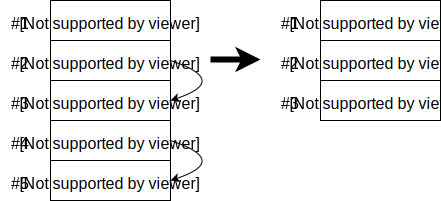
\includegraphics[scale=0.15]{Tail-compression.png}
  \end{figure}
\end{frame}

\begin{frame}
  \frametitle{Results}

  \only<1>{\begin{center}
    \scalebox{0.5}{%
    \begin{tabular}{|l|c|c|c|}
      \hline
      \multicolumn{4}{|c|}{LLC Load Misses (millions):}\\
      \hline
      \textbf{Name}&\textbf{Baseline}&\textbf{Tail-copy}&\textbf{Tail-compact}\\
      Allocate       &3.9     &+5.5\%         &+6.2\%         \\
      BinTree        &60.9    &-4.5\%         &-4.9\%         \\
      Bush           &33.5    &+4.1\%         &+2.8\%         \\
      BushTail       &50.9    &+0.8\%         &+0.6\%         \\
      Imbalanced     &40.9    &-10.3\%        &-11.0\%        \\
      MemBench       &84.1    &-80.3\%        &-80.0\%        \\
      PowerSet       &130.3   &-78.7\%        &-78.7\%        \\
      \hline
      \hline
      \multicolumn{2}{|l|}{Min}&-80.3\%&-80.0\%\\
      \multicolumn{2}{|l|}{Max}&5.5\%&6.2\%\\
      \multicolumn{2}{|l|}{Mean}&-23.3\%&-23.6\%\\
      \hline
    \end{tabular}}
  \end{center}}

  \only<3>{\begin{center}
    \scalebox{0.5}{%
    \begin{tabular}{|l|c|c|c|}
      \hline
      \multicolumn{4}{|c|}{Heap size:}\\
      \hline
      \textbf{Name}&\textbf{Baseline}&\textbf{Tail-copy}&\textbf{Tail-compact}\\
      Allocate       &1.8 gb         &+0.0\%         &-8.3\%         \\
      BinTree        &1.8 gb         &+0.0\%         &-6.2\%         \\
      Bush           &1.3 gb         &+0.0\%         &-3.1\%         \\
      BushTail       &5.1 gb         &+0.0\%         &-1.7\%         \\
      Imbalanced     &1.6 gb         &+0.0\%         &-6.2\%         \\
      MemBench       &6.7 gb         &+0.0\%         &-5.0\%         \\
      PowerSet       &10.4 gb        &+0.0\%         &-5.0\%         \\
      \hline
      \hline
      \multicolumn{2}{|l|}{Min}&0.0\%&-8.3\%\\
      \multicolumn{2}{|l|}{Max}&0.0\%&-1.7\%\\
      \multicolumn{2}{|l|}{Mean}&0.0\%&-5.0\%\\
      \hline
    \end{tabular}}
  \end{center}}

  \only<2>{\begin{center}
    \scalebox{0.5}{%
    \begin{tabular}{|l|c|c|c|}
      \hline
      \multicolumn{4}{|c|}{Branch Misses (millions):}\\
      \hline
      \textbf{Name}&\textbf{Baseline}&\textbf{Tail-copy}&\textbf{Tail-compact}\\
      Allocate       &3.7     &-6.1\%         &-13.8\%        \\
      BinTree        &29.0    &+107.5\%       &+102.5\%       \\
      Bush           &17.4    &+78.3\%        &+77.0\%        \\
      BushTail       &16.2    &+44.4\%        &+44.2\%        \\
      Imbalanced     &39.4    &+6.7\%         &+4.3\%         \\
      MemBench       &10.7    &-7.9\%         &-12.8\%        \\
      PowerSet       &20.0    &-6.7\%         &-10.7\%        \\
      \hline
      \hline
      \multicolumn{2}{|l|}{Min}&-7.9\%&-13.8\%\\
      \multicolumn{2}{|l|}{Max}&107.5\%&102.5\%\\
      \multicolumn{2}{|l|}{Mean}&30.9\%&27.3\%\\
      \hline
    \end{tabular}}
  \end{center}}

  \only<4>{\begin{center}
    \scalebox{0.5}{%
    \begin{tabular}{|l|c|c|c|}
      \hline
      \multicolumn{4}{|c|}{GC times:}\\
      \hline
      \textbf{Name}&\textbf{Baseline}&\textbf{Tail-copy}&\textbf{Tail-compact}\\
      Allocate       &1.5s           &+14.5\%        &+3.1\%         \\
      BinTree        &4.6s           &+16.2\%        &+10.2\%        \\
      Bush           &2.8s           &+12.5\%        &+9.6\%         \\
      BushTail       &3.6s           &+10.7\%        &+5.9\%         \\
      Imbalanced     &4.0s           &-0.7\%         &-6.2\%         \\
      MemBench       &7.8s           &-27.5\%        &-31.4\%        \\
      PowerSet       &12.6s          &-31.1\%        &-34.5\%        \\
      \hline
      \hline
      \multicolumn{2}{|l|}{Min}&-31.1\%&-34.5\%\\
      \multicolumn{2}{|l|}{Max}&16.2\%&10.2\%\\
      \multicolumn{2}{|l|}{Mean}&-0.8\%&-6.2\%\\
      \hline
    \end{tabular}}
  \end{center}}

  \begin{itemize}
    \item<1-> Mostly fewer LLC misses (-80\% to +6\%)
    \item<2-> More complex algorithm $\Rightarrow$ more branch misses
    \item<3-> 5.0\% smaller heap on average
    \item<4-> Four programs are slower and three are faster.
  \end{itemize}

\end{frame}

\begin{frame}
    \frametitle{Conclusion}
    \begin{enumerate}
        \item Reasonable implementation complexity? Yes.
        \item Improved performance? Mixed performance.
        \item Modern, fully-featured collectors? Unlikely.
    \end{enumerate}
\end{frame}


%\begin{frame}
    \frametitle{State Machine Design}
    \begin{figure}
      \begin{center}
        \includegraphics[height=0.7\textheight]{StateMachine.png}
      \end{center}
    \end{figure}
\end{frame}

%\begin{frame}
    \frametitle{Physics}
    \begin{itemize}
        \item Gravity equation: $ v(t_1) \approx a(t_0) \times \Delta t + v(t_0)$
        \item Gravity as a strategy / SOLID
        \item Playability: Ceiling on speed from gravity
        \item Thrusters can apply force left, right and up but not down
        \item Forces are defined as screen sizes per tick
        \item Thrust force is 0.01\% screen height/width per tick${}^2$
        \item Gravity is 0.005\% screen height per tick${}^2$
    \end{itemize}
\end{frame}

%\begin{frame}
    \frametitle{Collision Detection}
    \begin{itemize}
        \item StateMachine responsible for acting on collisions
        \item High level API in Level class (checks for collisions with walls and platforms)
        \item StateMachine responsible for collision logic
        \item StateMachine responsible for making platforms solid
    \end{itemize}
\end{frame}

%\begin{frame}
    \frametitle{Scoring points}
    \begin{itemize}
        \item Customers spawn after the player enters a level with a delay
        \item Score class can render itself
        \item StateMachine updates the score state
        \item Room for just 1 customer per trip
    \end{itemize}
\end{frame}

%\begin{frame}
    \frametitle{Level classes layout}
    \begin{figure}
      \begin{center}
        \includegraphics[height=0.7\textheight]{LevelUML.png}
      \end{center}
    \end{figure}
\end{frame}

%\begin{frame}
    \frametitle{Use case analysis}
    \begin{figure}
      \begin{center}
        \includegraphics[height=0.7\textheight]{UseCase.png}
      \end{center}
    \end{figure}
\end{frame}


%\begin{frame}
    \frametitle{Parser implementation}
    \pause
    \begin{itemize}
        \item No parser library
        \pause
        \item Repeated sanity checks
        \pause
        \item Edge-cases and maintainability
    \end{itemize}
\end{frame}

%\begin{frame}[fragile]
    \frametitle{Parser implementation}

\begin{lstlisting}
Name = Prefixed("Name: ", ExpectLine(lines));

string platformsLine = Prefixed("Platforms: ", ExpectLine(lines));
Platforms = platformsLine.Split(
              new[] {", "},
              StringSplitOptions.None);
\end{lstlisting}
\end{frame}


%\begin{frame}
    \frametitle{Testing}
    \begin{enumerate}
        \item White box, unit testing
        \begin{itemize}
          \item Correctness check for level 1 and 2
          \item Error handling checks
          \item Full coverage checks for customer parsing
        \end{itemize}
        \item Black box, integration testing
        \begin{itemize}
          \item Compile and run game
          \item Navigate entire state machine
          \item Collect and deliver customers
          \item Crash into walls
        \end{itemize}
    \end{enumerate}
\end{frame}

%\begin{frame}
    \frametitle{Improvements}
    \begin{itemize}
        \item Parsing (Parseq, Parsley, Pidgin)
        \item Bitmap Collision detection
        \item State machine tests
        \item Customer animations
        \item Additional maps
    \end{itemize}
\end{frame}

%\begin{frame}
    \frametitle{Gameplay}
    \begin{figure}
      \begin{center}
        \includegraphics[height=0.7\textheight]{GamePlay.png}
      \end{center}
    \end{figure}
\end{frame}


\end{document}



% Hi, my name is David. Today I'll be talking about my bachelor work
% on cache optimizations in a semi-space garbage collector.
% My work started out with an idea that a garbage collector could,
% in certain situations, arrange heap objects differently
% in order to make better use of CPU caches. I'll explain the details shortly.
% ------- FLIP SLIDE --------
% In my bachelor project, I wanted not only to verify that my idea could make
% a garbage collector faster but also to get an objective measure of its
% implementation complexity and whether it could be expected to work in a
% modern collector. You see, the garbage collector I'll be using as a baseline
% is quite simple and doesn't support mutable objects and it is not generational.
% ------- FLIP SLIDE --------
% First a little background. Why are garbage collectors interesting? Well, of
% the 10 most popular languages on GitHub,
% ------- FLIP SLIDE --------
% 8 of them are garbage collected. This usually means the programmers of these
% languages do not get to decide precisely how their data is arranged in memory.
% ------- FLIP SLIDE --------
% Does this matter? Does it matter how data is arranged in memory? Isn't memory
% random-access and therefore has a constant latency and bandwidt? It does matter
% because the abstraction of random-access memory is leaky. Some memory requests
% will be served from the cache, some from physical memory, others possibly from a swap
% file on disk. Furthermore, the different layers have different chunk sizes.
% Caches can be accessed word-by-word but physical memory is accessed in chunks
% of usually 8 words at a time.
% This means data arrangement has an effect on both data bandwidth
% and data latency.
% ------- FLIP SLIDE --------
% The type of garbage collector I'll be working with is called a semi-space
% garbage collector. The collector works by traversing live objects and copying
% them to a separate space. It was first described by Fenichel who used a
% depth-first algorithm to traverse the object graph. But depth-first traversal
% requires stack space to keep track of which objects are yet to be copied and
% this limited the possible size of the heap. One year later, Cheney realized
% that a breadth-first algorithm could use the 'to-space' to keep track of which
% objects to copy, thus supporting arbitrarily large heaps. This style of
% garbage collection has become widely used,
% especially among functional programming languages that allocate lots of
% short-lived objects and require high garbage collection through-put.
% ------- FLIP SLIDE --------
% This figure shows in which order the objects are copied.
% The move away from depth-first copying was a mixed blessing. CPU
% caches make it several times cheaper to access objects if they're close
% together and depth-first copying is really good at this, always placing
% branches next to each other.
% ------- FLIP SLIDE --------
% Breadth-first copying, on the other hand, tends to intersperse data and put
% unrelated objects together.
% ------- FLIP SLIDE --------
% For example, object 5 and 6 only share a grandparent but they're put right
% next to each other. Even worse, if we add another branch to the
% root node, that branch will be interpersed with the previous branches.
% ------- FLIP SLIDE --------
% Now we finally get to the first on my two ideas. Is there a way to traverse
% the object graph which does not require any stack, which does not require
% any reserved heap, and which has a higher likelihood of placing related
% objects close together?
% ------- FLIP SLIDE --------
% It's possible to deeply copy a single branch of each node and then use
% breadth-first copying for all the other branches without requiring any stack.
% This leads to smaller chunks of continuous memory where objects have a parent
% to child relation. This alone should improve performance in some situations.
% ------- FLIP SLIDE --------
% Now on to the second idea.
% Given that many parent-child pairs are placed right next to each other, the
% pointer between them contains no useful information and can be replaced by
% a single tag bit. If the bit is set, the pointer is omitted and the child
% must be right below the parent. This should save heap space and lead to less
% copying.
% There are several corner cases, such as objects with multiple parents or
% objects that were copied before their parents, which must all be accounted
% for.
% ------- FLIP SLIDE --------
% I've implemented these two ideas in the LHC Haskell Compiler and benchmarked
% them with 7 test programs.
% A key metric is last-level-cache misses. This is how often a memory request
% has to go all the way to physical memory. Here, tail copying does extremely
% well and only struggles slightly on two programs. Tail compaction is a marginal
% improvement on top of this.
% ------- FLIP SLIDE --------
% Identifying the special cases where the two methods can be applied is not
% free and there are three programs which are seriously hampered by failed
% branch prediction. A branch miss will stall the CPU and can be as expensive
% as a cache miss.
% Interesting enough, tail-compaction has to check if a parent is compacted
% before accessing the child. I thought this check would be expensive but
% it turns out to be completely inconsequential. The CPU is able to predict
% it well.
% ------- FLIP SLIDE --------
% One large benefit of tail compaction is that programs take up less space.
% How much space is saved depends on the data and the allocation patterns
% but it tends to be a significant amount. In the benchmarks, it saved 5 percent
% on average.
% It should be noted that I'm not using the saved space to make the collections
% run faster. To get comparible results, each garbage collector has the same
% allocation area and runs the same number of times.
% ------- FLIP SLIDE --------
% The total garbage collection time is influenced primarily by cache misses and
% branch misses. As such, only three of the seven programs see an actual
% performance gain. BinTree, Bush and BushTail are all held back for the same
% reason: excessive number of branch misses.
% Allocate is a bit of a special case with fewer
% branch misses but more cache misses.
% ------- FLIP SLIDE --------
% Does the implementation have a reasonable complexity? Yes, it only take up
% 10% of the RTS.
% Is the performance improved? Only in some cases. In future work, it may be
% possible to only
% enable the optimizations for certain data types and thereby limit the
% downsides. It's also possible to use the saved heap space to make collection
% a little bit faster.
% Can these optimizations be used in a modern collector? As it stands, I think
% not.
% Modern collectors support mutable objects and are often generational. Both
% these things interfere with my two optimizations and would make the benefits
% even less pronounced.

%
